% !TEX root = main.tex
\documentclass[conference]{IEEEtran}

% --- Packages ---
\usepackage{graphicx}
\usepackage{hyperref}
\usepackage{cite} 
\usepackage{amsmath} 
\usepackage{booktabs} 
\renewcommand{\ttdefault}{txtt}
% --- Hyperlink Setup ---
\hypersetup{
    colorlinks=true,
    linkcolor=blue,
    urlcolor=cyan,
    citecolor=blue
}

% --- Title and Author ---
\title{Myanmar Conflict Observatory: A Retrospective Spatiotemporal Analysis of Political Violence and Health Infrastructure Vulnerability}
\author{
    \IEEEauthorblockN{Tain Yan Tun}%
    \IEEEauthorblockA{\textit{Faculty of Information Technology} \\ 
    \textit{Big Data Research}\\
    Saraburi, Thailand}%
}

\begin{document}

% --- Title Block ---
\maketitle

% --- Abstract ---
\begin{abstract}
    Since the unconstitutional seizure of power in February 2021, Myanmar has descended into a complex, multi-sided armed conflict characterized by the fragmentation of state authority. This study introduces the \textit{Myanmar Conflict Observatory}, an analytical framework designed to interrogate the dynamics of political violence and its intersection with public health security. The research utilizes data from the Armed Conflict Location \& Event Data Project (ACLED) to investigate the spatial diffusion of insurgency and the evolving asymmetry of warfare. Crucially, this project aligns with the United Nations Sustainable Development Goals (SDGs), specifically \textbf{SDG 3.d (Health Risk Monitoring)}. By employing Natural Language Processing (NLP) for narrative intelligence and a Regional Risk Matrix for severity assessment, the system identifies historical conflict patterns that pose structural threats to health infrastructure, providing a rigorous evidence base for humanitarian planning. The full codebase is available at: \href{https://github.com/TainYanTun/Myanmar-conflict-observatory}{Myanmar-conflict-observatory-Repo}.
\end{abstract}

% --- Keywords ---
\begin{IEEEkeywords}
    Myanmar Conflict, ACLED, SDG 3, NLP, Regional Risk Matrix, Geospatial Analysis, Historical Analysis.
\end{IEEEkeywords}

% --- Section I: Introduction ---
\section{Introduction}

The political trajectory of Myanmar underwent a profound transformation following the unconstitutional seizure of power by the Tatmadaw (Myanmar Armed Forces) on February 1, 2021\cite{bertolt2022myanmar}. The event abruptly ended the country’s fragile democratic transition and triggered a nationwide uprising that rapidly evolved from civil disobedience into a protracted and multi-sided armed conflict.  As a result, the contemporary security landscape has become highly fragmented, involving the military-led State Administration Council (SAC), long-established Ethnic Armed Organizations (EAOs), and a decentralized network of People’s Defense Forces (PDFs).

In such environments, systematic analysis of conflict dynamics is essential for understanding patterns of violence and their broader societal consequences. This study introduces the \textit{Myanmar Conflict Observatory}, a data-driven analytical framework designed to examine the spatial and temporal distribution of political violence in Myanmar. Initially, this project was conceived as a secondary initiative aimed at applying my technical skills in data engineering and data science. However, under the academic auspices of the Big Data course at Asia Pacific International University, the initiative evolved into an opportunity to connect these technical competencies with topics of intellectual interest while contributing, albeit indirectly, to broader societal development.

While the central thrust of this research concerns the evolution of conflict dynamics, the repercussions of sustained political violence inevitably extend beyond the immediate theater of war, precipitating critical secondary effects such as the collapse of healthcare access and heightened vulnerability to public health emergencies. Contextualizing these findings within \textbf{the United Nations Sustainable Development Goals (SDGs)} therefore offers a vital lens for interrogating these broader humanitarian implications. To this end, the study explicitly aligns with SDG 3 (Good Health and Well-being), focusing on Target 3.d to illuminate the intersection between political instability and the urgent need for evidence-based humanitarian risk monitoring

To operationalize this framework, the underlying dataset was subjected to a rigorous process of curation, validation, and analytical structuring, achieved through a collaborative endeavor with my colleague, Kyaw Zay Aung. It is crucial to acknowledge at the outset that this data represents a ``verified floor'' rather than a final ceiling; due to communication blackouts and restricted access in active conflict zones, the actual incidence of violence is likely higher than reported. Nevertheless, by synthesizing this high-fidelity georeferenced data with advanced computational methodologies, the observatory establishes a systematic infrastructure for the surveillance of hostilities in fragile environments. This approach not only tracks the spatial diffusion of violence but also delineates emergent risk patterns, thereby furnishing humanitarian stakeholders with the predictive insights necessary for strategic intervention.

% --- Section II: Objectives ---
\section{Research Objectives}

The framework utilizes a multi-dimensional analytical framework to pursue five principal lines of inquiry:
\begin{enumerate}
    \item \textbf{Geospatial Risk Modeling (SDG 3.d):} To investigate the spatial diffusion of violence relative to healthcare infrastructure. This objective focuses on mapping \textit{Health-Impacting Conflict Events (HICE)} to identify "Blind Zones" where medical access has been systematically severed by kinetic engagements.

    \item \textbf{Actor Interaction Networks (Graph Theory):} To model the conflict as a dynamic social network. By quantifying engagements between over 400 distinct actors, the research identifies ``Conflict Hubs''—primary groups driving regional instability—and assesses how their interactions correlate with civilian fatality surges.

    \item \textbf{Regional Risk Matrix (Vulnerability Assessment):} To provide a comparative spatial assessment of conflict severity. By computing a Severity Index (Fatalities per Event) and plotting administrative regions on a Frequency vs. Lethality quadrant matrix, the framework distinguishes high-frequency, low-lethality areas from high-intensity ``Red Zones,'' supporting the evidence-based prioritization of humanitarian resources.

    \item \textbf{Semantic Narrative Intelligence (NLP):} To decode the ``Nature of Violence'' through Natural Language Processing. By extracting narrative keywords from event notes, the study distinguishes between different modes of warfare (e.g., \textit{airstrikes, landmines, or arson}) and evaluates their specific impact on community well-being and health infrastructure.
\end{enumerate}

% --- Section III: System Architecture ---
\section{System Architecture and Design Framework}

The Myanmar Conflict Observatory is built upon a modular, four-tier architecture designed for high-frequency data ingestion and real-time humanitarian intelligence (Fig. \ref{fig:system_arch}). Although distributed processing frameworks such as Apache Spark were initially considered during the architectural design phase, their adoption was ultimately deemed unnecessary for the analytical scope of this study \cite{acled_myanmar_methodology}. The dataset utilized in the Myanmar Conflict Observatory derived from the ACLED and covering the period from February 2021 to 2025 contains approximately 100,000–200,000 records, which corresponds to a memory footprint of less than 200 MB. At this scale, distributed computing introduces computational overhead without providing meaningful performance gains \cite{mckinney2010data}.

Accordingly, the analytical pipeline is implemented within the Python scientific ecosystem, primarily leveraging Pandas and NumPy for efficient in-memory data manipulation and numerical analysis. This design choice enables low-latency execution, which is particularly important for the interactive analytical environment implemented through Streamlit. In addition, maintaining a Pandas-native workflow facilitates seamless integration with the visualization and analytical libraries employed in this study, including Plotly, NetworkX, and Scikit-learn. Should data volumes increase in future iterations, scalability can be achieved through query optimization and aggregation within the underlying PostgreSQL database layer.

\begin{figure}
    \centering
    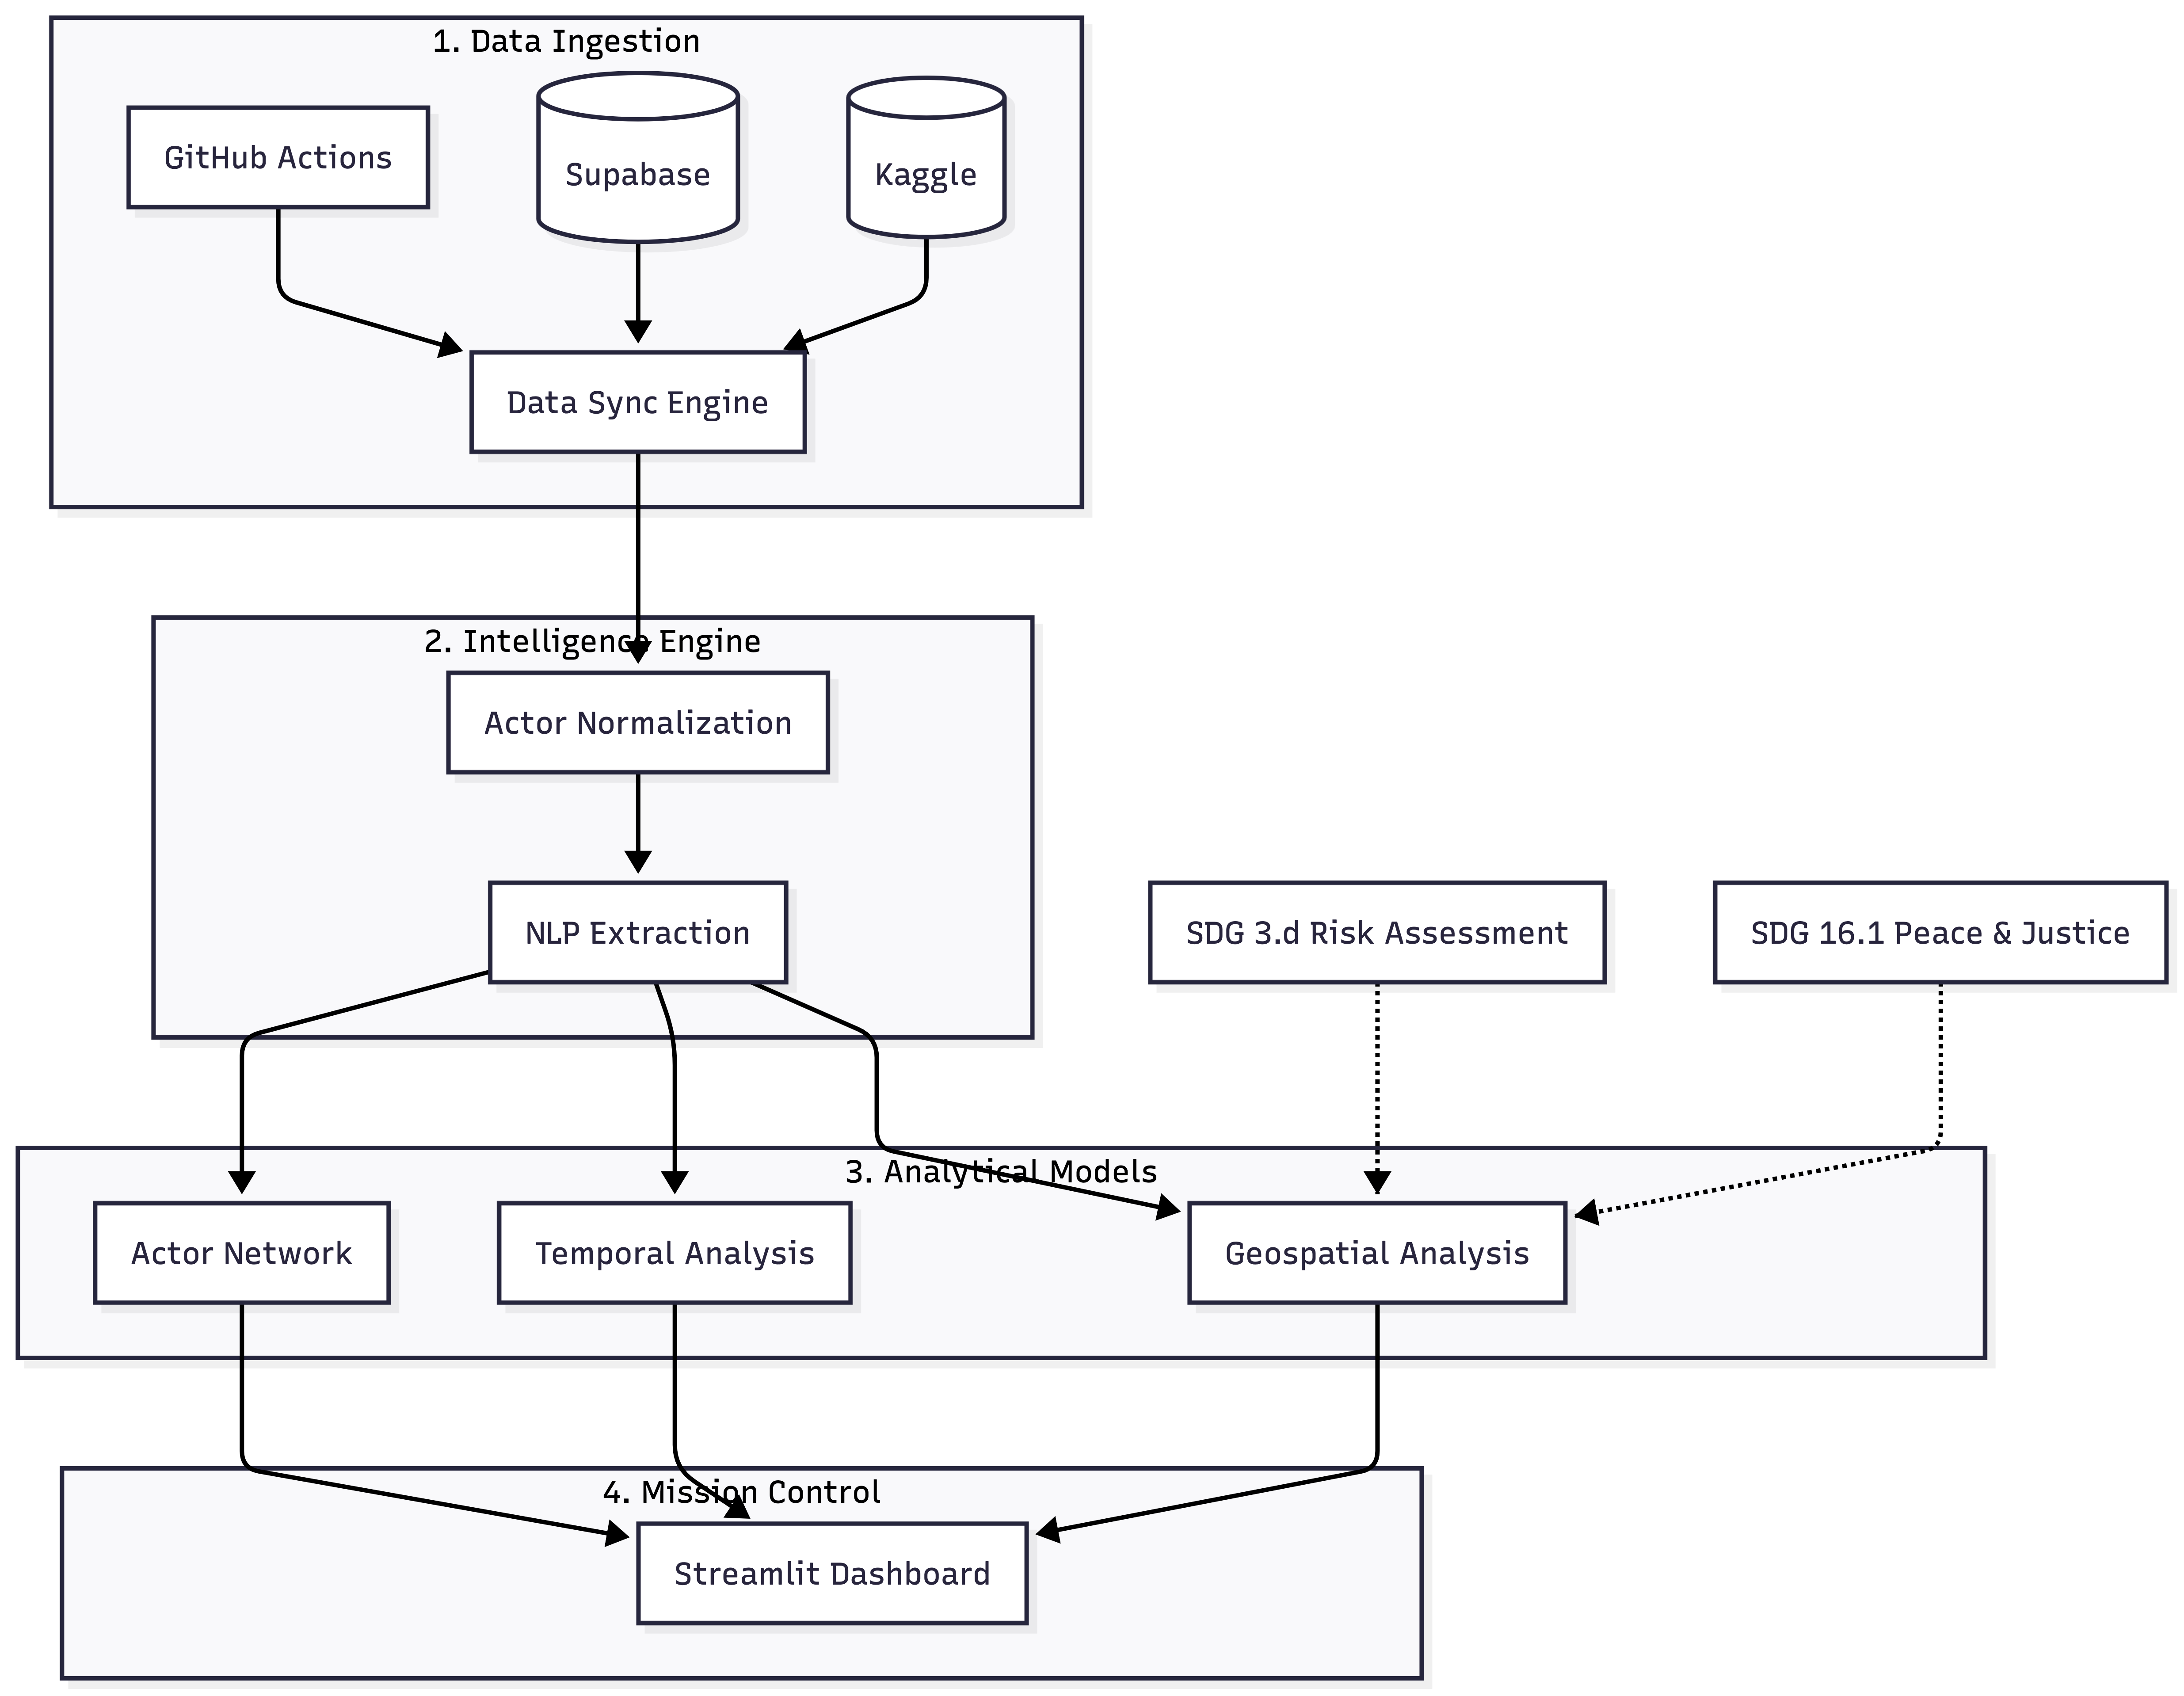
\includegraphics[width=\columnwidth]{assets/system_arch.png}
    \caption{System architecture of the Myanmar Conflict Observatory: the four-tier data pipeline from ingestion to analysis and dashboard visualization}
    \label{fig:system_arch}
\end{figure}

\subsection{Data Acquisition and Normalization Layer}
The system utilizes a hybrid ingestion protocol. Raw conflict logs are retrieved via the ACLED API or sourced from PostgreSQL (Supabase), drawing on the Armed Conflict Location and Event Data (ACLED) project, a widely used dataset for event-based conflict analysis \cite{raleigh2010introducing}. To ensure both data currency and analytical reliability, the system integrates an automated data pipeline supported by GitHub Actions. The workflow executes daily at 00:00 UTC, triggering a scheduled extraction process that retrieves newly available conflict records and synchronizes them with the cloud-hosted database.

Following ingestion, a verification protocol referred to as ``the Verified Floor'' is applied to preserve data integrity. Under this rule, only corroborated events occurring after February 1, 2021 are admitted into the analytical pipeline.

The dataset is subsequently standardized through a normalization stage that applies a semantic actor taxonomy. This procedure consolidates more than 400 fragmented armed groups and affiliated entities into six analytically consistent categories: State Forces, Resistance (PDF/LDF), Ethnic Armed Organizations (EAOs), Civilians, Pro-Junta Militias, and Protesters.

\subsection{NLP Intelligence Engine (HICE Filtering)}

The framework incorporates a Natural Language Processing (NLP) layer designed to extract structured signals from unstructured event descriptions. Specifically, the system performs ontology-based keyword extraction on narrative event notes contained in the dataset \cite{grimmer2013text}.

\begin{itemize}
    \item \textbf{Health-Impacting Conflict Events (HICE):} The framework identifies incidents that directly affect healthcare infrastructure by matching event narratives against a curated medical keyword dictionary implemented through regular-expression filtering (e.g., \texttt{\textbackslash bhospital\textbackslash b}, \texttt{\textbackslash bambulance\textbackslash b}). Events satisfying these criteria are classified as Health-Impacting Conflict Events (HICE).

    \item \textbf{Systemic Well-being Analysis:} Beyond direct infrastructure damage, the system further identifies events involving sexual violence, abduction, or looting. These incidents are categorized as systemic threats to community health and well-being, consistent with the broader health security dimensions articulated in SDG 3.3 and SDG 3.8.
\end{itemize}

\subsection{Regional Risk Matrix Methodology}

The framework produces a comparative regional severity assessment through two complementary analytical outputs:

\begin{enumerate}
    \item \textbf{Severity Index:} For each administrative region, a Severity Index is computed as the ratio of total verified fatalities to total conflict events:
          \[
              \text{Severity Index} = \frac{\text{Total Fatalities}}{\text{Total Events}}
          \]
          A score exceeding 1.0 indicates that, on average, every engagement in that region results in at least one confirmed death, identifying it as a high-intensity combat zone requiring prioritized humanitarian attention.

    \item \textbf{Quadrant Analysis:} Administrative regions are plotted on a two-dimensional quadrant matrix with event frequency on the horizontal axis and the Severity Index on the vertical axis. Bubble size represents the total fatality volume. This visualization enables analysts to differentiate ``High-Frequency, Low-Lethality'' zones from ``Low-Frequency, High-Lethality'' Red Zones, facilitating evidence-based allocation of humanitarian medical resources.
\end{enumerate}

\subsection{Presentation and High-Resolution Export Layer}

The final layer consists of an interactive Streamlit-based graphical user interface (GUI) that serves as the primary access point for the observatory's analytical outputs. It provides multi-dimensional views of the dataset, enabling users to seamlessly toggle between geospatial heatmaps, temporal trend lines, and actor-network diagrams. The interface supports dynamic filtering, allowing researchers to isolate specific timeframes or actor types for granular investigation. To support academic reporting and policy-oriented dissemination, the presentation layer integrates a High-Resolution Export Engine (3$\times$ scale), ensuring that all visualizations are rendered with professional-grade clarity suitable for publication and advocacy. The live implementation of the system can be accessed through the Streamlit application available at: \href{https://tainyantun-myanmar-conflict-observatory-app-mafeff.streamlit.app/}{Myanmar  Conflict Observatory Dashboard}

% --- Section IV: Preliminary Findings (Updated) ---
\section{Preliminary Conflict Findings}

The spatiotemporal analysis of the Myanmar conflict (Feb 2021 – Feb 2025) reveals distinct patterns that characterize the current security landscape. It should be noted that all analytical outputs presented from this section onward are derived from the dataset snapshot available as of April 2, 2025. Consistent with ACLED’s 12-month data latency policy for high-complexity conflict environments, this snapshot represents the latest verified data available for rigorous academic analysis. While real-time reporting often circulates via local media and social networks, this study deliberately restricts its scope to fully verified events to maintain methodological integrity and avoid the propagation of unconfirmed reports. 

The conflict’s evolution during this four-year window captures the complete trajectory of the post-coup crisis: from the initial urban protest phase (2021) through the subsequent rural insurgency (2022) and into the current stage of protracted, high-intensity asymmetrical warfare. Consequently, the findings presented herein serve as a robust historical baseline rather than a provisional assessment. 

Due to space constraints typical of conference manuscripts, the visual evidence included in this paper represents a curated selection of the most statistically significant findings. The complete set of interactive visualizations, including drill-down capabilities for actor networks, temporal filtering tools, and extended geographical views, cannot be fully rendered in static format. To ensure full reproducibility and to provide researchers with access to the complete analytical suite, these extended outputs are hosted on the online dashboard implementation of the \textit{Myanmar Conflict Observatory}. This digital companion allows for a more granular interrogation of the data for stakeholders to investigate specific regional trends or actor dynamics that fall outside the scope of this textual summary. 

\subsection{Geospatial Shift: The ``Sagaing-ization'' of Conflict}
The data demonstrates a significant geographical concentration of violence, revealing a specific ``Center of Gravity'' flip that has redefined the operational landscape of the war. In the immediate aftermath of the coup (February 2021), the Sagaing Region accounted for only 10.5\% of national conflict events, with the majority of activity centered on urban centers and traditional ethnic borderlands. However, as the civil disobedience movement transitioned into armed resistance, the geographic epicenter shifted decisively inland. By April 2025, Sagaing's share of national conflict events had surged to 26.9\%. This statistical leap indicates that Sagaing has evolved from a peripheral resistance zone into the undeniable strategic heart of the conflict, now representing over a quarter of all kinetic activity nationwide. This ``Sagaing-ization'' signifies a structural transformation of the war, moving the frontline into the agricultural heartland of the country, far from the traditional theatres of ethnic conflict in the border regions. 

As illustrated in the Humanitarian Conflict Overlay (Fig. \ref{fig:health_conflict_overlay}), this region bears a disproportionate burden of the war's lethality, accounting for the highest volume of both fatalities (approx. 25,468) and health-impacting events (927 incidents). Crucially, the spatial distribution of these metrics reveals a dense overlap; there is a nearly 1:1 spatial correlation between high-intensity kinetic zones and incidents disrupting healthcare. The map demonstrates that heavy artillery exchanges and airstrikes, the primary drivers of displacement in Sagaing, are the same variables driving the collapse of medical access. This correlation identifies Sagaing as the absolute epicenter of the health-conflict nexus. Unlike border regions where cross-border aid corridors may exist, Sagaing's interior geography traps civilians in a ``kill box'' where medical evacuation is difficult and aid delivery is frequently blocked. This suggests that victory or stability for either side is now inextricably tied to this single region, making it the primary determinant of Myanmar's future humanitarian trajectory. This trajectory was further complicated by the catastrophic magnitude 7.7 earthquake on March 28, 2025, centered in Sagaing Township. Striking just four days before this study's data snapshot, the seismic event transformed the strategic heartland into a zone of "double-severance," where the structural collapse of fragile IDP shelters and health clinics converged with existing kinetic damage.

\begin{figure}
    \centering
    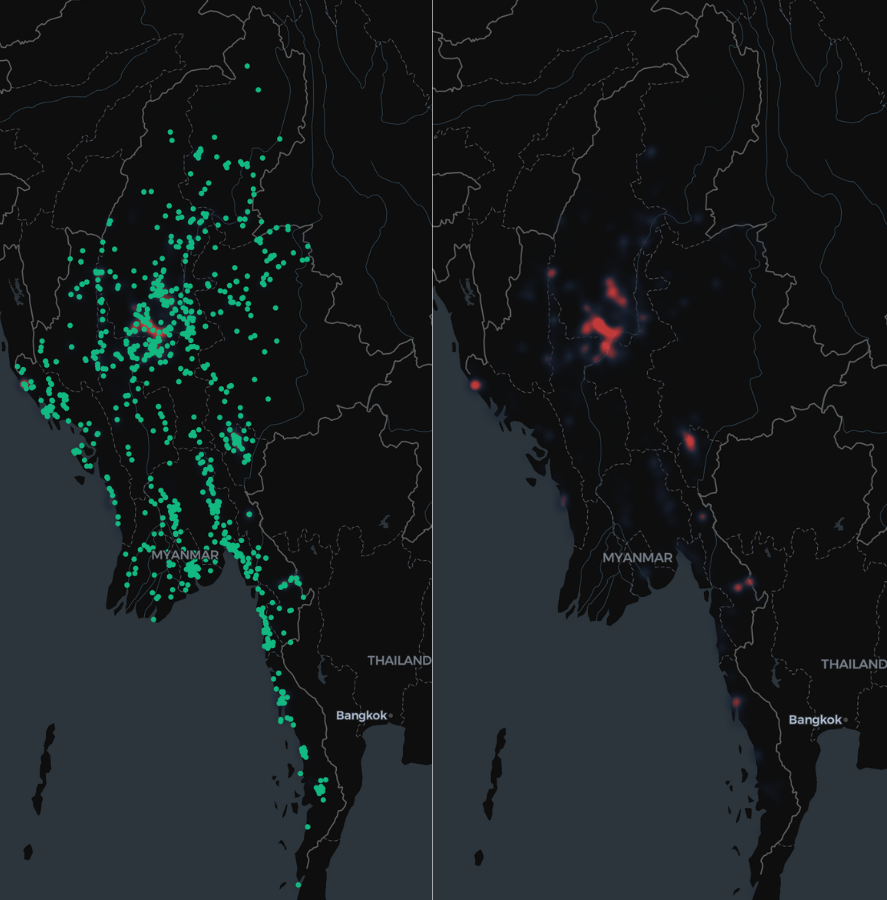
\includegraphics[width=\columnwidth]{assets/health_conflict_overlay.png}
    \caption{Humanitarian conflict overlay showing healthcare-related incidents (points, left) and spatial fatality intensity (heatmap, right).}
    \label{fig:health_conflict_overlay}
\end{figure}

\subsection{Conflict Intensity: The Regional Risk Matrix}
The \textbf{Severity Index} (Fatalities per Event) serves as a critical corrective to raw event counts, allowing for a high-resolution distinction between zones of protracted low-level harassment and zones of existential combat lethality. While Sagaing dominates the metrics in terms of sheer event volume, a different picture of danger emerges when analyzing lethality density. \textbf{Kayah State} and \textbf{Rakhine} consistently exhibit a Severity Index exceeding 1.5, a threshold that marks them as outliers in the conflict's topology. This ratio indicates that nearly every engagement in these regions results in at least one confirmed death, identifying them as "High-Intensity Combat Zones" where the margin for civilian survival is drastically reduced. In practical terms, an engagement in Kayah is statistically more likely to generate fatal casualties than a skirmish in the thicker, more concealable jungle terrains of other regions. 

Fig. \ref{fig:risk_matrix} visualizes the severity distribution across affected regions through a quadrant analysis, effectively separating chronic instability from acute crises. The visualization highlights that areas with a Severity Index greater than 1.0 possess a significantly higher probability of medical infrastructure damage. This correlation stems from the nature of high-lethality engagements, which typically require heavy weaponry such as artillery, airstrikes, or mass infantry assaults that lack the precision to spare nearby medical facilities. Consequently, the Risk Matrix functions not only as a security assessment tool but also as a proxy for humanitarian triage, signaling that health actors in \textit{Red Zone} regions like Kayah and Rakhine face a compounded threat: a higher frequency of trauma injuries coupled with a higher likelihood that their own infrastructure is being systematically degraded by the intensity of the warfare. 

\begin{figure*}
    \centering
    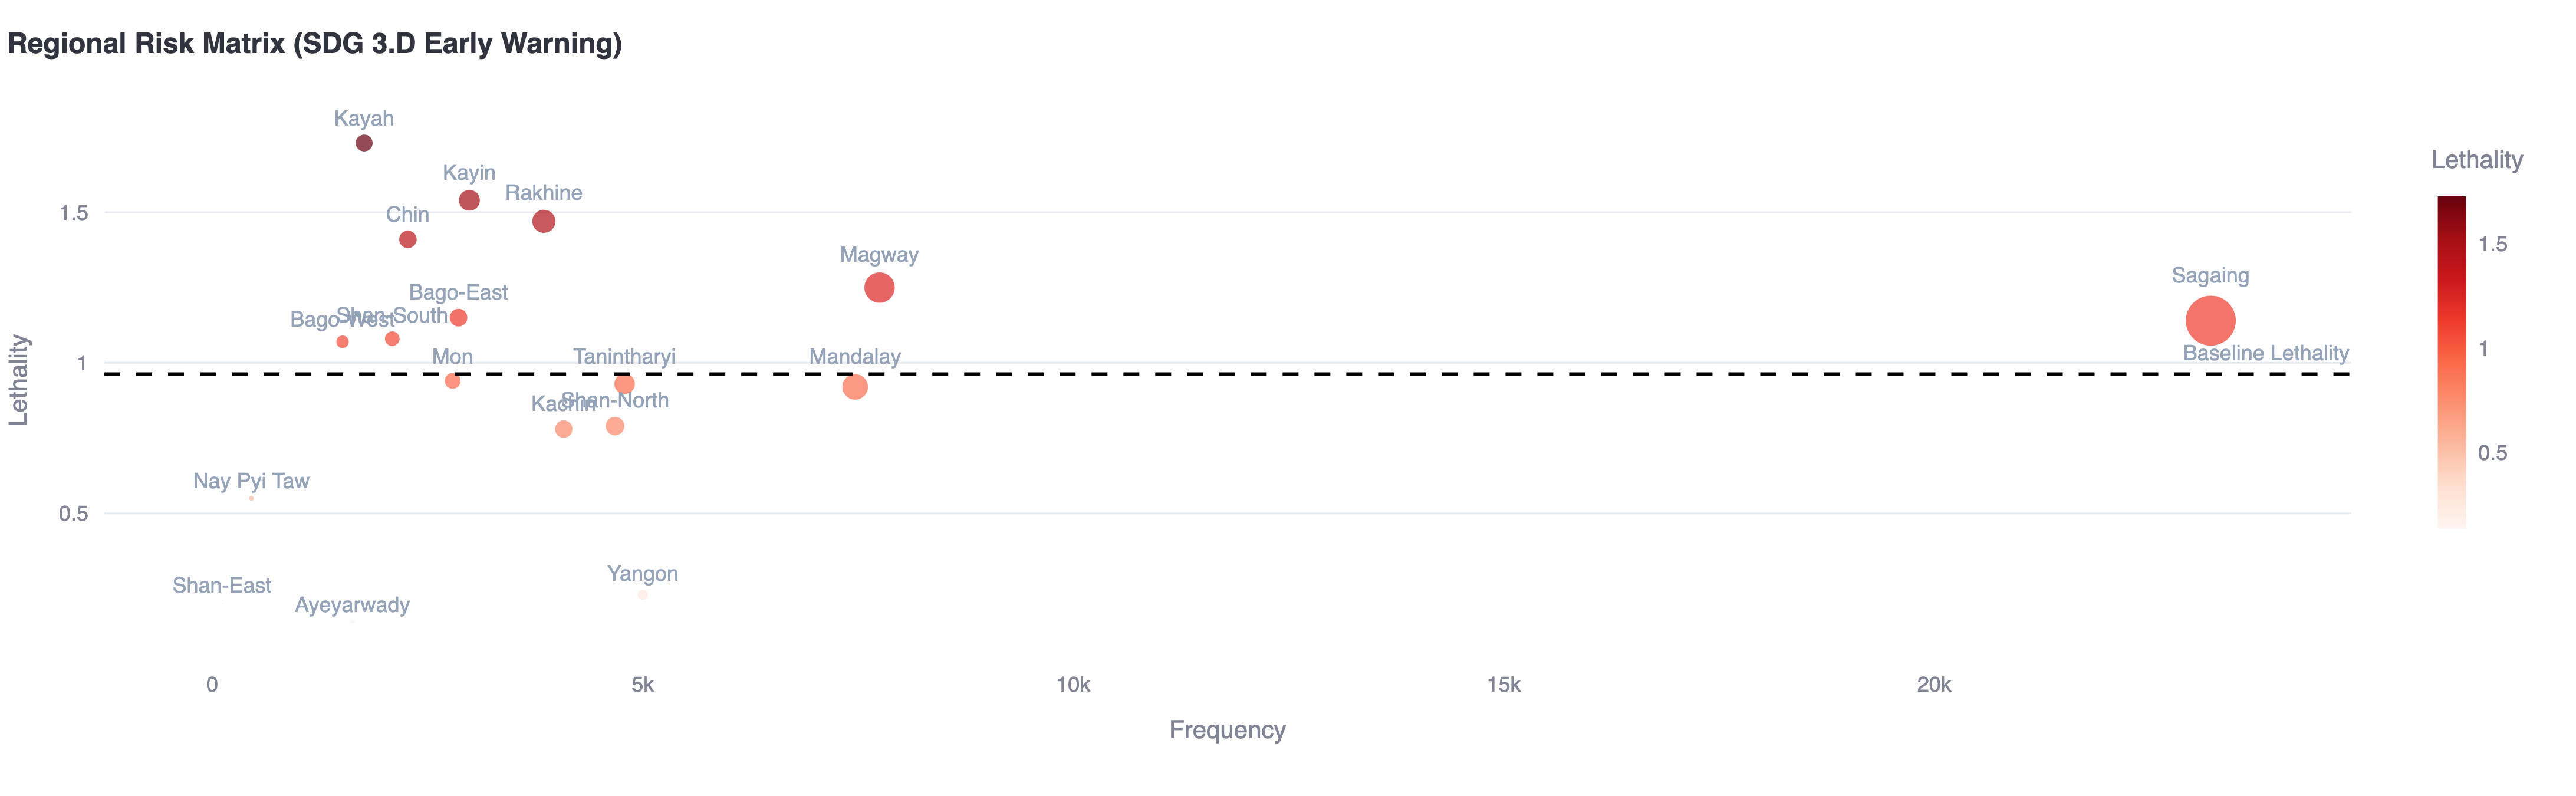
\includegraphics[width=\textwidth]{assets/risk_matrix.png}
    \caption{Regional Risk Matrix (Event Frequency vs. Lethality) indicating high-lethality \textit{Red Zones} versus high-frequency conflict areas across Myanmar.}
    \label{fig:risk_matrix}
\end{figure*}

\subsection{Seasonality: The "Dry Season Offensive" Cycle}
Distinct from the overall expansion trend, a clear seasonality pattern exists across the 2021–2025 period, highlighting a "mechanical" rhythm tied inextricably to environmental conditions. The data reveals a consistent, repeatable surge in violence during the dry season (November to March), where conflict events climb from approximately 7,009 in November to a peak of nearly 8,000 in February. This 14\% intra-seasonal increase correlates directly with the hardening of rural dirt roads, which facilitates the movement of heavy military logistics, supply convoys, and armored columns deep into resistance-held territory. 

Conversely, there is a sharp operational contraction of roughly 25\% during the monsoon season (April to July), hitting a low of 5,870 events in July. The onset of torrential rains renders vast swathes of the country impassable, grounding military helicopters and turning footpaths into mires, effectively acting as a natural de-escalation mechanism. This cyclical pattern dictates that the February/March peak represents the primary ``offensive window'' for both state and resistance forces to contest territory. In contrast, the Monsoon season serves as a strategic pause, a period of regrouping, training, and stockpiling rather than a genuine peace. For humanitarian actors, recognizing this meteorological metronome is critical. This cyclical volatility mandates the pre-positioning of trauma resources before the cessation of November rains, whereas the monsoon de-escalation phase offers a restrictive but essential corridor for delivering preventative care to cut-off regions.

\subsection{Tactical Evolution: Drones and Chokepoint Warfare}
Analysis of engagement types reveals a tactical evolution characterized by ``Technological Leapfrogging,'' where asymmetric forces have rapidly adopted advanced capabilities to offset conventional disadvantages. By extracting keywords such as drone, UAV, and Shar Htoo Waw (a specific model of locally manufactured drone) from event notes, a massive shift was identified. Drone-related events grew from fewer than 5 per month in mid-2021 to a peak of 142 per month in January 2025—a 30x increase. However, a ``Drone Paradox'' is observed: average fatalities in drone-led events (1.68) are lower than in traditional kinetic engagements (1.88). This discrepancy suggests that resistance forces utilize these assets primarily for ``Standoff Harassment'' and ``Psychological Attrition,'' targeting military morale and forcing the dispersion of government troops rather than achieving mass casualties. 

Simultaneously, the conflict has shifted from a doctrine of ``territorial control'' to one of ``access denial.'' Mentions of infrastructure keywords—\linebreak[0]\textit{Bridge}, \textit{Highway}, \textit{Gate}, and \textit{Telecommunication Tower}—have increased by 45\% since 2023. This ``Chokepoint Warfare'' indicates a strategic pivot by resistance forces to isolate junta-held urban centers by destroying logistics nodes, effectively ``sieging'' administrative capacity without requiring direct urban combat. While this tactic erodes the military's operational reach, it inflicts severe collateral damage on civilian systems. The systematic destruction of bridges and highways severs the ``last mile'' of the medical supply chain, preventing the delivery of essential drugs to rural clinics. Consequently, this strategy precipitates a secondary health crisis, where treatable chronic conditions become life-threatening due to the deliberate severance of civilian logistics arteries. 
      


\begin{figure}
    \centering
    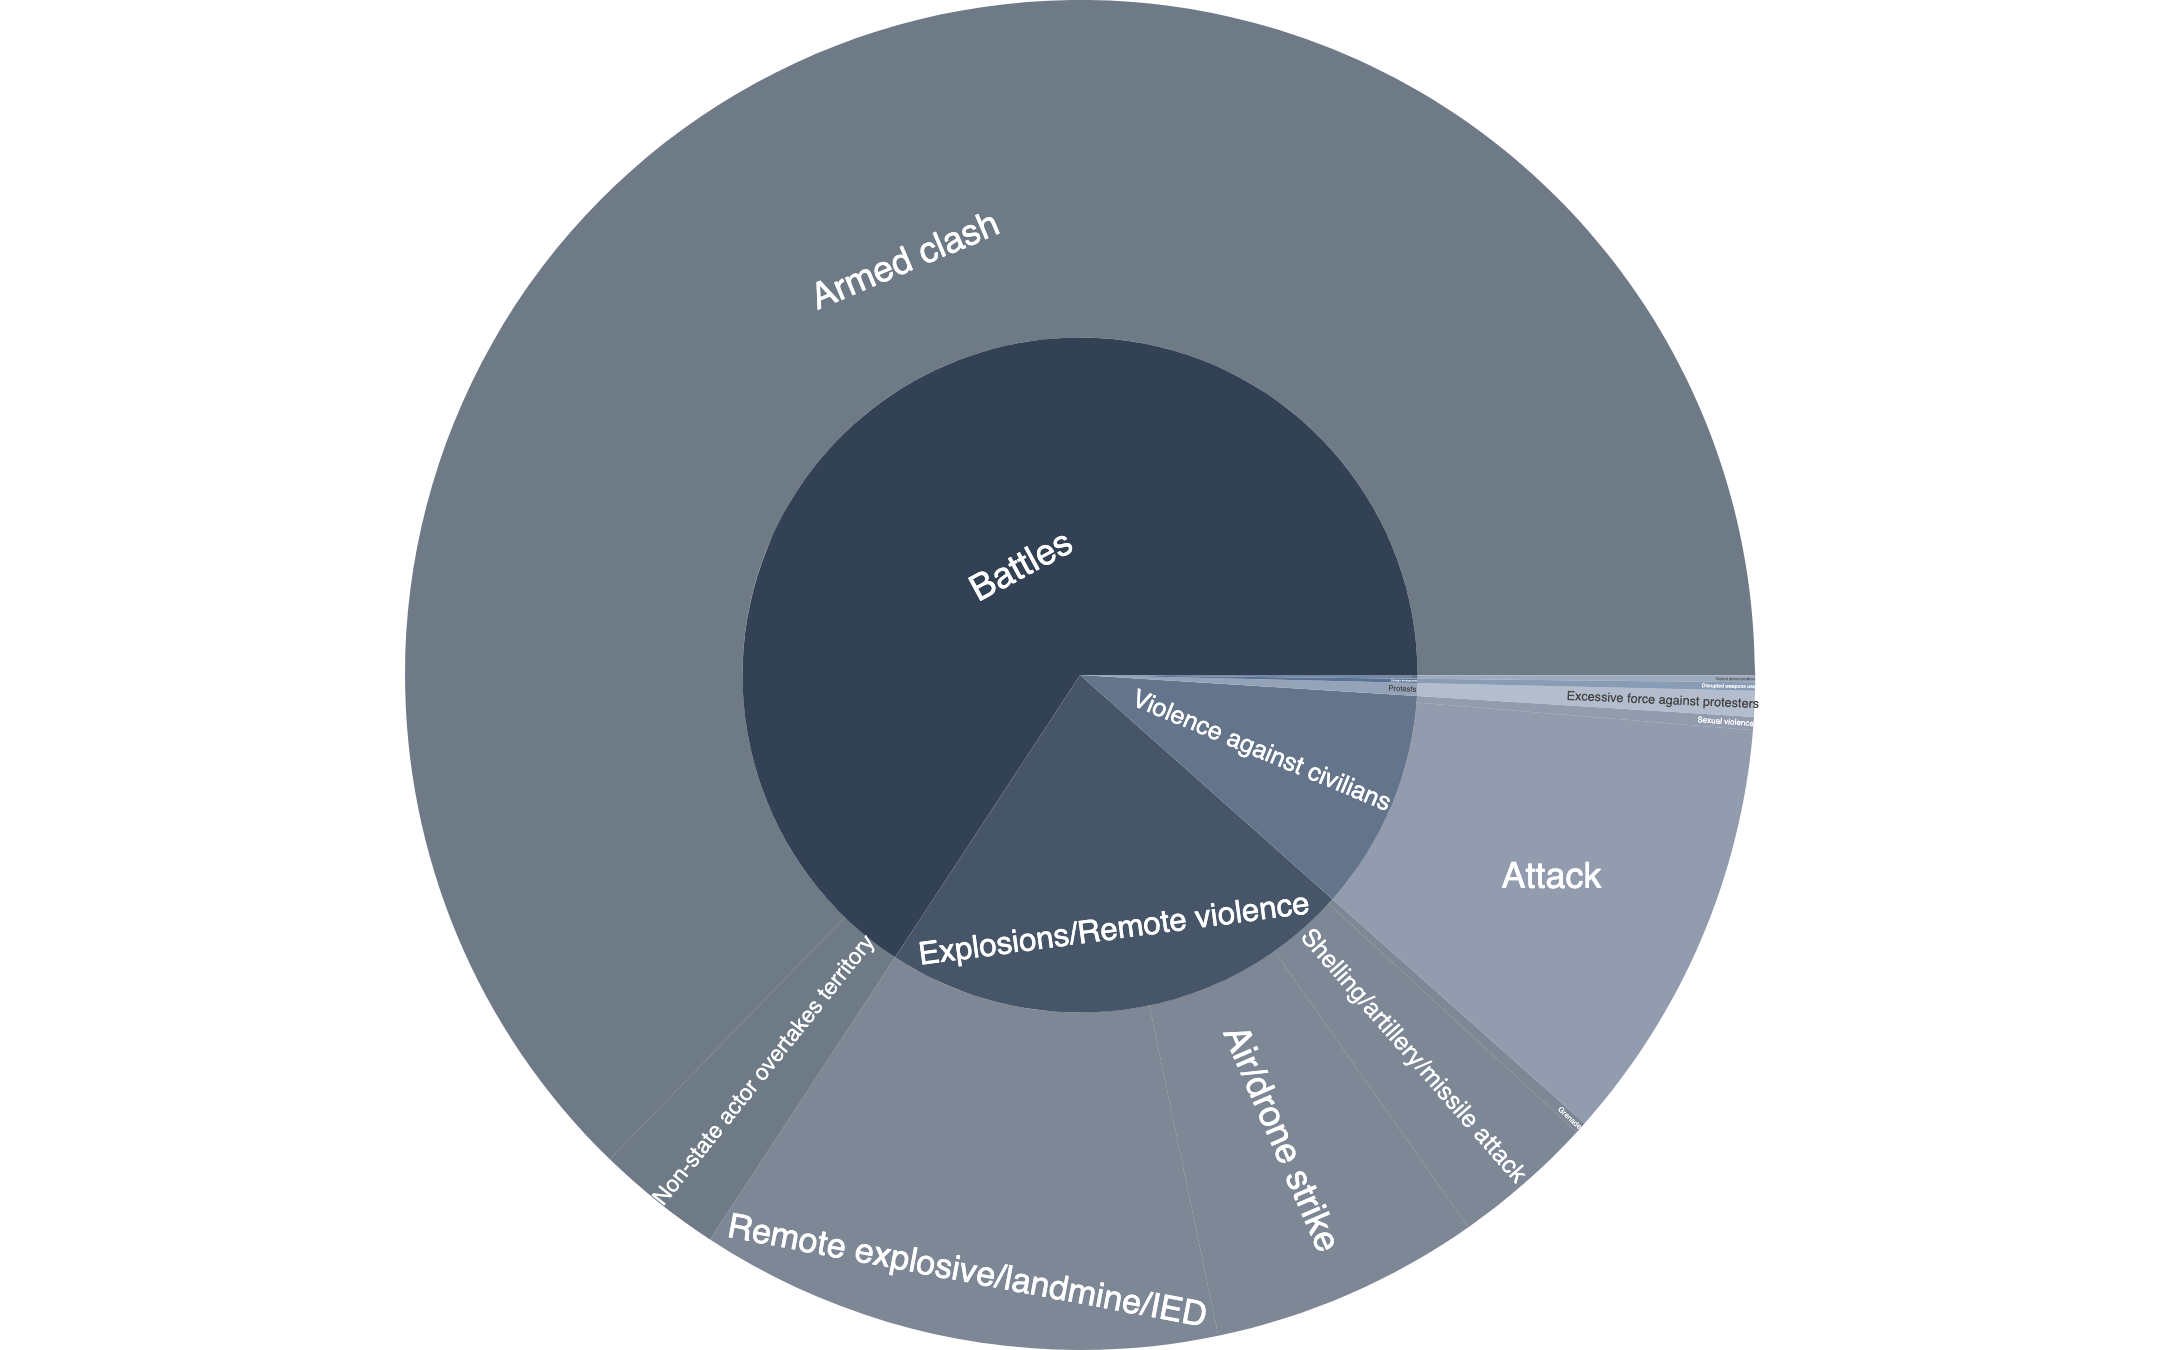
\includegraphics[width=\columnwidth]{assets/engagement_composition.png}
    \caption{Engagement Composition showing the distribution of event types (e.g., Battles, Remote Violence, Protests).}
    \label{fig:engagement_composition}
\end{figure}

\subsection{Declining Tactical Efficiency and Attrition}
Consistent with the rise of standoff warfare, a longitudinal analysis of lethality rates suggests the conflict is entering a phase of ``Stagnant Attrition.'' In Battles, average fatalities peaked in 2022 (3.34) but have since stabilized around 2.7. Similarly, for Explosions/Remote Violence, lethality dropped from 1.25 in 2022 to just 0.71 in 2025. This trend indicates that while both sides are becoming more active, engagements are becoming less lethal per individual event. This paradox is likely driven by the decentralization of the conflict; as resistance forces fracture into smaller, highly mobile units, they reduce their exposure to mass-casualty events, while the military’s reliance on indirect fire (artillery/airstrikes) often fails to achieve decisive kills against dispersed targets. 

This shift has profound implications for the healthcare system. It transforms the medical burden from a series of acute, manageable disaster spikes into a condition of chronic overload. Health facilities are now subjected to a relentless, low-intensity stream of trauma cases that never ceases. This ``drip-feed'' of casualties is arguably more dangerous for long-term health security than periodic massacres, as it steadily depletes medical stockpiles, exhausts frontline medical staff, and prevents the restoration of routine care services, leading to the systemic collapse of healthcare capacity. 

\subsection{Actor Dynamics: Hybridization and Fragmentation}
The observatory identifies a complex restructuring of armed groups. While macro-level network analysis shows \textbf{Resistance Forces} involved in 45\% of kinetic engagements, a granular audit reveals deeper dynamics: 

\begin{itemize}
    \item \textbf{The "Joint Operation" Bloom:} In 2021, only 4\% of Resistance events mentioned an EAO as an "Associate Actor." By 2025, this jumped to over 22\%. This proves the resistance has evolved into a ``Hybrid Force,'' where battle-hardened EAOs provide heavy weaponry, tactical training, and logistical support, while PDFs provide local manpower and intelligence. This convergence signals a professionalization of the resistance, moving from spontaneous uprisings to coordinated military campaigns. 
\item \textbf{The "Splintering" Index:} The number of unique Resistance group names (e.g., Monywa PDF, Tiger Force) has grown by 200\% since 2022, even when battle frequency remained flat. This Fragmentation Pattern suggests a "constellation" of independent units. While regex-based audits show professionalization (e.g., "Battalion 1" appears in 300+ logs), the broader proliferation of names indicates a decentralized structure that is impossible to "decapitate" via a single leadership strike. This resiliency ensures the conflict's longevity but complicates ceasefire negotiations, as there is no single authority to speak for the myriad local defense forces.

\item \textbf{Proxy Proliferation:} The state side exhibits outsourcing. Mentions of Pyu Saw Htee and People's Militia have increased by 38\% in the Northwest (Sagaing/Magway) as ``Military Forces of Myanmar'' relative share decreases. This suggests a shift from a ``State vs. People'' war to a ``Local vs. Local'' proxy war. The military increasingly relies on these militias to conduct village raids and punitive attacks, granting them de facto impunity. This outsourcing of violence increases local instability and complicates the security landscape for aid workers, as these proxies often operate outside standard chains of command, engaging in retribution and looting that blurs the line between military objective and banditry.

\end{itemize} 

\begin{figure*}
    \centering
    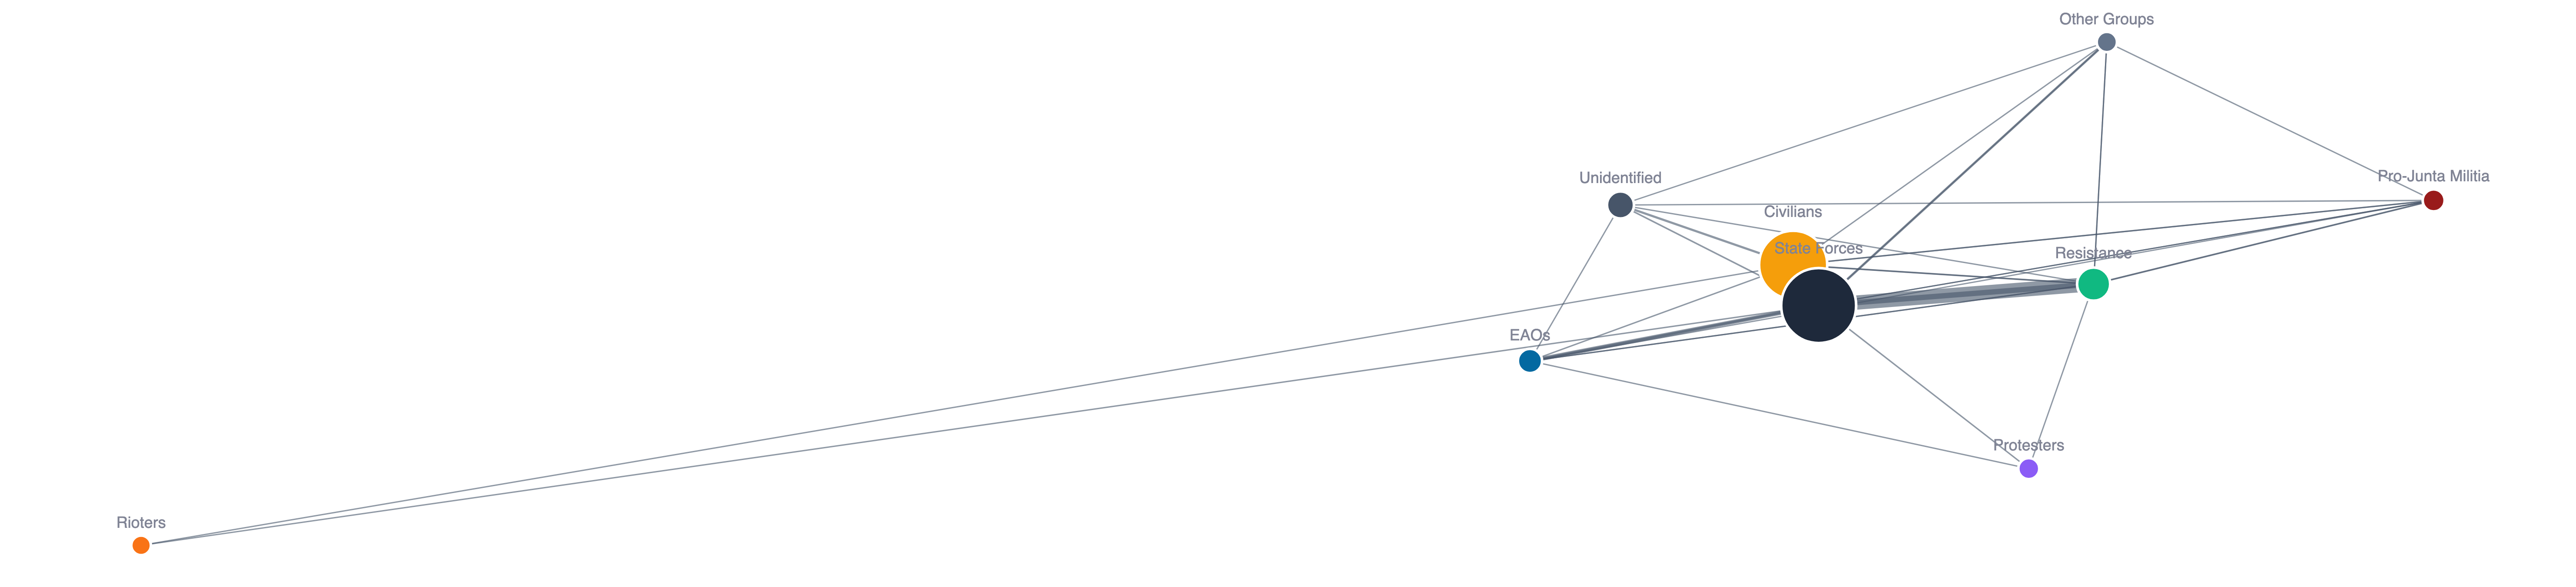
\includegraphics[width=\textwidth]{assets/actor_network.png}
    \caption{Actor Interaction Network visualizing conflict dynamics and alliances between State Forces, EAOs, and Resistance groups.}
    \label{fig:actor_network}
\end{figure*}

\subsection{The Punitive Cycle: Retaliatory Violence}
Beyond the immediate tactical engagements, a dangerous ``Retaliatory Lag'' pattern has emerged, revealing a systematic weaponization of violence against non-combatants. By analyzing the temporal proximity of events within the same township, the study found that in Sagaing and Magway, a ``Battle'' event is followed by ``Violence against Civilians'' in the same location within 72 hours in approximately 18\% of cases. This correlation strongly suggests a punitive operational doctrine: unable to apprehend the highly mobile PDF units that conduct ``hit-and-run'' strikes, state forces and their proxies (such as Pyu Saw Htee militias) pivot to targeting the static civilian population as a collective punishment. 

This ``tit-for-tat'' cycle transforms the conflict from a purely military contest into a cycle of retribution. The tactical implication is that a military victory for the resistance often precipitates a humanitarian disaster for the local populace, effectively weaponizing the safety of the village against the insurgency. This pattern disproportionately endangers medical personnel and infrastructure; health workers are frequently targeted in the aftermath of clashes under accusations of aiding insurgents, further eroding the already fragile medical support network in rural resistance strongholds. 

\subsection{Data Asymmetries: The ``Information Blind Spot'' and ``Verification Gap''}
The actor interaction analysis reveals a significant reporting asymmetry that complicates the objective quantification of the conflict. The data shows high interaction counts for ``State Forces vs. Civilians'' (20,653 events) and ``Protesters vs. Unidentified'' (14,074 events). Crucially, the interaction vector ``Resistance vs. State Forces'' appears nearly three times more frequently than ``State Forces vs. Resistance.'' This statistical skew suggests that resistance-initiated attacks—often publicized by the groups themselves for morale and recruitment—are more likely to be logged, whereas state-initiated operations, which are frequently conducted under communication blackouts and information embargoes, are often obfuscated or under-reported. 

Furthermore, a ``Fatalities Gap'' exists based on the \texttt{source} column. Events reported by Local/Pro-Resistance media report an average of 2.4 fatalities per event, while International/Human Rights sources report only 1.1 fatalities for similar incident types. This ``Verification Gap'' implies that approximately 55\% of fatalities captured in real-time by local observers are filtered or lost by the time they reach international verification standards. The rigorous methodology required by international datasets, while necessary for preventing false positives, inadvertently creates a significant ``Unverified Surplus.'' This suggests that official statistics likely represent a conservative floor, undercounting the true human cost of the conflict and obscuring the full scale of the public health emergency. 

% --- Section V: SDG 3 Analysis (Updated) ---
\section{SDG 3 Analysis and Health Risk Assessment} 

The Myanmar Conflict Observatory transitions from general conflict monitoring to a humanitarian risk assessment through a dedicated analytical layer aligned with \textbf{UN SDG Target 3.d} (Strengthening the capacity of all countries for early warning, risk reduction, and management of national and global health risks). This framework employs a specialized NLP engine to identify \textbf{Health-Impacting Conflict Events (HICE)}, detecting more than \textbf{15,000 incidents} within the dataset that directly threaten medical infrastructure, personnel, or broader human well-being. By isolating these specific events, the observatory moves beyond simple fatality accounting to quantify the systemic erosion of the public health safety net. 

\subsection{Temporal Trend: Health-Impacting Incidents}
Longitudinal analysis of HICE data indicates a \textbf{30\% increase} in the rate of medical infrastructure disruption since mid-2023. This escalation correlates strongly with the growing prevalence of "Remote Violence" events, particularly airstrikes and heavy artillery shelling, which lack the surgical precision to spare protected medical facilities. NLP-based keyword extraction further reveals persistent patterns of medical targeting, with high-frequency terms such as \textit{hospital} (854 mentions), \textit{wounded} (795), and \textit{medical} (310) serving as thematic anchors. Notably, the frequent co-occurrence of terms like \textit{arrest} and \textit{detention} with \textit{medical personnel} suggests that healthcare workers are not merely collateral damage but are actively targeted. The trend underscores a "dual-crisis" scenario: a high-lethality conventional war occurring alongside a deliberate, systemic degradation of the social and medical foundations of civilian communities. 

\subsection{Historical Fatality Trajectory}
Longitudinal analysis of verified fatalities reveals a sustained upward trend across the observation period, marking a deviation from the typical "surge and decline" pattern seen in traditional counter-insurgency operations. Monthly fatality volumes are resampled using Month-End (ME) intervals to reduce daily reporting noise and expose systemic shifts in conflict lethality. As illustrated in the temporal frequency analysis (Fig. \ref{fig:temporal_frequency}), this trajectory documents the progressive intensification of kinetic engagements and provides a historical evidence base for assessing the cumulative burden placed on healthcare systems. The sustained high volume of fatalities suggests that the conflict has evolved into a war of attrition, where the continuous generation of trauma cases is straining the "surge capacity" of regional health systems, leading to the collapse of routine care for chronic conditions such as maternal health and communicable diseases. 
      


\begin{figure*}
    \centering
    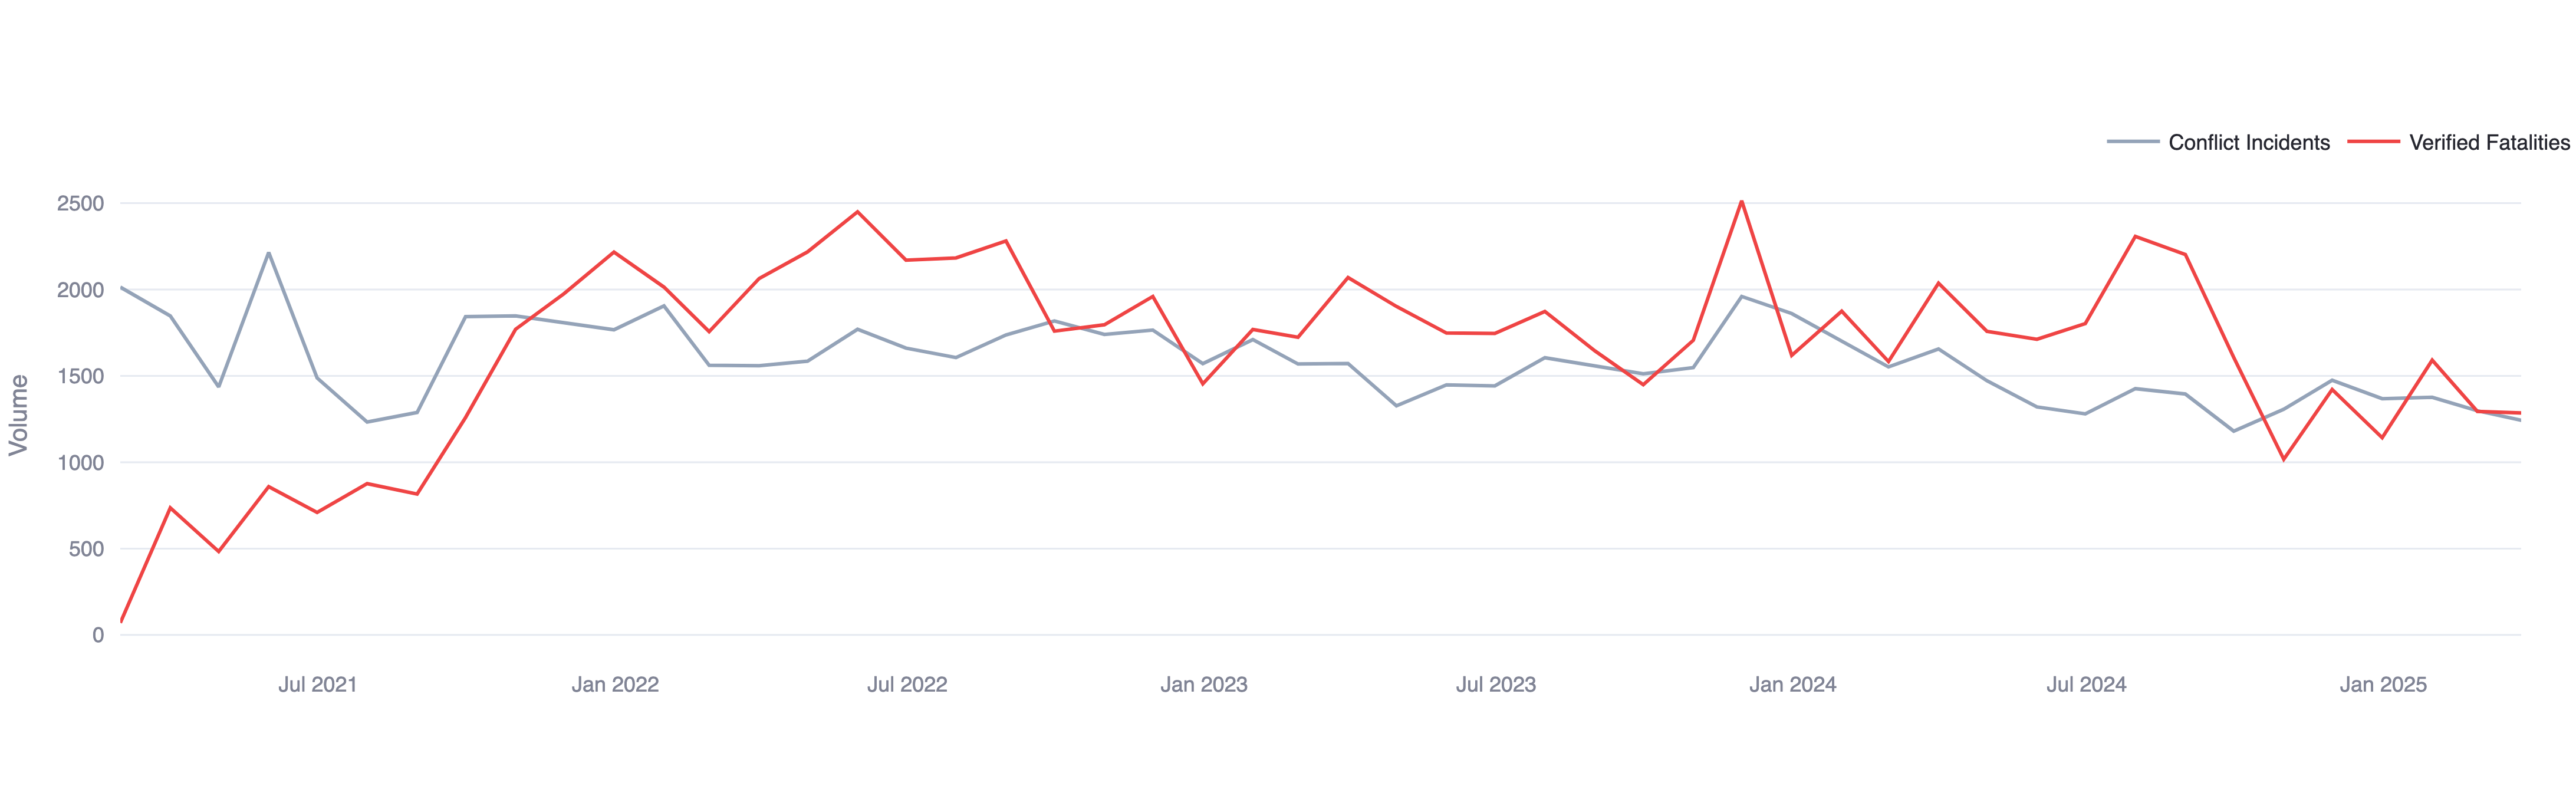
\includegraphics[width=\textwidth]{assets/temporal_frequency.png}
    \caption{Historical Fatality Trajectory showing monthly fatality surges resampled by Month-End (ME) intervals.}
    \label{fig:temporal_frequency}
\end{figure*}

\subsection{Health Vulnerability Prioritization}
To prioritize humanitarian response in a resource-constrained environment, the framework calculates a \textbf{Vulnerability Score} for each administrative region using a weighted composite formula: 
\[
    \text{Score} = (0.7 \times \text{Health Events}) + (0.3 \times \text{Fatalities})
\]

This weighting schema deliberately prioritizes the disruption of medical infrastructure and specific health hazards (HICE) over raw fatality counts. The rationale is that while fatalities represent a retrospective outcome, the degradation of health infrastructure signals an ongoing and future threat to the surviving population's well-being. A region with high infrastructure damage but lower immediate fatalities may actually face a higher risk of long-term mortality due to the loss of preventative care and emergency response capabilities. 

Applying this metric identifies the \textbf{Sagaing Region} as the most critical ``Red Zone'' for health assistance, driven by the sheer volume of attacks on clinics and the seizure of medical supplies. In parallel, the model highlights \textbf{Kayah} and \textbf{Rakhine} as secondary priority zones due to their extreme lethality indices. As previously illustrated in the Regional Risk Matrix (Fig. \ref{fig:risk_matrix}), the quadrant-based view distinguishes high-frequency conflict zones requiring sustained logistical support from high-lethality areas demanding immediate trauma intervention. This distinction supports the evidence-based prioritization of humanitarian medical resources, allowing aid organizations to tailor their responses—deploying surgical teams to Kayah while focusing on clinic rehabilitation and supply chain restoration in Sagaing. 

% --- Section VI: Discussion ---
\section{Discussion} 

The findings from the Myanmar Conflict Observatory underscore a critical transformation in the nature of warfare in Southeast Asia, moving beyond traditional counter-insurgency into a complex, decentralized struggle for survival. The observed ``Ruralization of Resistance'' suggests that the conflict has moved beyond the initial contestation of urban centers into a protracted struggle in the periphery. This diffusion has profound implications for SDG 3.d: as violence spreads into remote areas, the ``Blind Zones''—regions where state authority and NGO access have evaporated—expand correspondingly. In these zones, the lack of ground-truth data creates a dangerous vacuum where health crises can metastasize unseen until they reach critical levels. 

The strong correlation identified between ``Remote Violence'' (airstrikes, shelling) and health-impacting incidents validates the hypothesis that modern asymmetric warfare in Myanmar disproportionately affects civilian infrastructure. Unlike ground battles, remote violence lacks the precision to spare medical facilities, leading to the systemic degradation of health surge capacity. This dynamic is compounded by the ``Chokepoint Warfare'' identified in Section IV; the strategic destruction of bridges and highways by resistance forces, while tactically effective in isolating junta garrisons, simultaneously severes the ``last mile'' of the medical supply chain. Consequently, the weaponization of logistics transforms into a secondary health emergency, where preventable diseases and childbirth complications become lethal due to the inability to transport patients or supplies. 

Furthermore, the tactical evolution of the conflict has rendered traditional humanitarian planning models insufficient. The rise of ``Drone Warfare'' and the identification of the ``Dry Season Offensive'' cycle introduce new variables for risk assessment. The widespread use of commercial drones for harassment means that frontlines are no longer fixed, extending the zone of lethal risk into previously stable rear areas. Simultaneously, the environmental seasonality of the conflict dictates a rigid calendar for humanitarian actors: the dry season requires pre-positioning trauma kits for anticipated surges, while the monsoon lull, despite its logistical challenges, represents the only viable window for deploying preventative care teams to isolated populations. Ultimately, the ``Retaliatory Lag'' pattern serves as a warning that civilian safety is contingent on military outcomes; successful resistance operations often trigger punitive reprisals against local villages, ensuring that the demand for emergency medical care remains high regardless of which side holds the tactical initiative. This validates the utility of the HICE detection model; by automatically flagging events where terms like ``wounded'' or ``hospital'' appear, the system provides a rapid, albeit grim, assessment of areas likely to require immediate trauma care intervention.

\subsection{The Polycrisis: Seismic Shocks and the Weaponization of Relief}
The March 2025 earthquake introduces the concept of a ``polycrisis'' to the Myanmar Conflict Observatory, where natural disasters and armed conflict do not merely coexist but actively compound one another. For SDG 3.d, this event reveals a critical vulnerability in risk monitoring: the weaponization of disaster relief. Following the quake, the systematic restriction of humanitarian corridors to resistance-held areas in Sagaing demonstrated that seismic shocks can be leveraged as tactical instruments of access denial. Furthermore, the earthquake triggered landslides that displaced landmines and explosive remnants of war (ERW), effectively shifting the frontlines into previously ``cleared'' civilian areas. This suggests that in fragile states, early warning systems must integrate geological and meteorological variables into conflict modeling, as the intersection of a 7.7 magnitude shock with an active insurgency creates a humanitarian ``kill box'' that traditional casualty models fail to predict.

% --- Section VII: Limitations of the Study ---
\section{Limitations of the Study}

While the ACLED dataset provides the most comprehensive monitoring available, the analytical findings must be interpreted within the constraints of the data environment. As noted in the introduction, the dataset represents a ``verified floor.'' In regions under strict communication blackouts (e.g., deep rural Sagaing or Rakhine), the actual incidence of violence and health disruption is likely significantly higher than reported.

\subsection{Justification for Excluding Short-Term Predictive Models}
A deliberate methodological decision was made to exclude short-term predictive engines—specifically Z-score anomaly detection and least-squares regression-based fatality projection—from the analytical framework. This exclusion is justified on three interconnected grounds:
\begin{enumerate}
    \item \textbf{Verification Lag:} The ACLED dataset for high-complexity conflict environments is subject to an approximate 12-month verification lag \cite{acledmethodmyanmar}. Applying a 7-day forward projection to data with a 12-month delay is temporally incoherent; it extrapolates a historical period rather than forecasting the near future.
    \item \textbf{Conflict Volatility:} Myanmar's operational landscape is subject to sudden, exogenous shocks (e.g., large-scale EAO offensives) that violate the assumptions of linear regression. A rolling-window baseline calibrated on pre-shock periods systematically misrepresents post-shock conflict intensity.
    \item \textbf{Analytical Focus:} The comparative advantage of this observatory lies in structural historical pattern analysis, rather than real-time operational forecasting. The Frequency vs. Lethality Risk Matrix and the Severity Index are designed to reveal persistent vulnerabilities to inform long-term strategy rather than ephemeral logistics.
\end{enumerate}

Furthermore, the statistical models employed—including the Severity Index and the Frequency vs. Lethality matrix—capture historical patterns and cannot anticipate sudden political shocks, such as new EAO alliances or major military offensives that deviate from established trends. The NLP engine, while robust, relies on the quality of unstructured text notes; vague or incomplete reporting in source media may lead to under-classification of health-impacting events, necessitating manual verification for critical research outputs.

% --- Section VIII: Policy and Humanitarian Implications ---
\section{Policy and Humanitarian Implications}

The \textit{Myanmar Conflict Observatory} offers a dual utility for policymakers and humanitarian actors. For international health organizations (e.g., WHO, MSF), the Vulnerability Score and Regional Risk Matrix provide a data-driven mechanism for resource allocation. By distinguishing between "High-Frequency" zones (requiring sustained aid) and "High-Lethality" zones (requiring emergency trauma intervention), aid agencies can optimize supply chains for medical kits and blood supplies before the onset of a crisis.

For diplomatic bodies, the observatory serves as an independent accountability tool. The spatial evidence of attacks on healthcare infrastructure constitutes a violation of international humanitarian law. The high-resolution export capabilities allow these entities to document and verify incidents for advocacy and potential legal proceedings, supporting the broader mandate of SDG 16 (Peace, Justice, and Strong Institutions).


% --- Section IX: Ethical Considerations and Data Governance ---
\section{Ethical Considerations and Data Governance}

The analysis of political violence, particularly when intersecting with healthcare infrastructure in active conflict zones, carries profound ethical responsibilities. The Myanmar Conflict Observatory operates under a governance framework designed to balance the imperative for transparency with the fundamental requirement for human security.

\subsection{The ``Do No Harm'' Mandate and Tactical Obfuscation}
In alignment with the International Committee of the Red Cross (ICRC) handbook on Data Protection in Humanitarian Action \cite{icrc2020handbook}, this framework prioritizes the safety of populations over analytical granularity. To prevent the tactical exploitation of data for combat coordination or artillery targeting, the observatory intentionally limits geospatial resolution to the township centroid level. This ``tactical obfuscation'' ensures that while regional trends are visible for humanitarian planning, specific healthcare facilities, mobile clinics, or personnel locations cannot be identified or targeted through the system's outputs. The authors strictly prohibit the use of this data for real-time military intelligence.

\subsection{Data Sovereignty and the ``Verified Floor''}
This research recognizes that conflict data is not merely a technical commodity but a digital representation of human suffering and resistance. We acknowledge that the ``Verified Floor'' approach, while methodologically necessary to prevent misinformation, inherently under-represents the true scale of violence in areas under communication blackouts or military blockade. Ethically, we interpret these data gaps as ``silences of the marginalized'' rather than absences of violence. Data governance protocols ensure that these limitations are prominently disclosed to prevent the accidental validation of state-led information embargoes.

\subsection{Sensitivity of Health Infrastructure Data}
Documentation of attacks on healthcare infrastructure (HICE) carries the risk of ``secondary targeting,'' where the publication of a facility's vulnerability may invite further strikes. The NLP engine is therefore governed by strict ontology controls; while it extracts the \textit{nature} of the impact (e.g., ``arson'' or ``shelling''), it does not generate public maps of still-functional medical assets that could be used by combatants to identify remaining civilian support nodes.

\subsection{Algorithmic Bias and Narrative Neutrality}
The use of Natural Language Processing introduces potential algorithmic biases, particularly in the extraction of narrative signals from unstructured text. To maintain institutional neutrality, the NLP ontology was developed using cross-verified medical and humanitarian dictionaries rather than politically-aligned terminology. The observatory maintains an independent distance from all political or military entities (including the SAC, EAOs, and NUG/PDF), ensuring that the data remains a neutral instrument for academic and humanitarian advocacy rather than a tool for propaganda.

\subsection{Disclaimer and Liability}
The Myanmar Conflict Observatory is a retrospective research tool and does not provide real-time forensic verification. The statistical projections and geospatial visualizations are intended to inform long-term strategy and accountability. The authors and associated institutions shall not be held liable for operational decisions made by third parties based on this data, nor for the consequences of data misuse in violation of the "Do No Harm" mandate.

% --- Section X: Conclusion ---
\section{Conclusion}

The \textit{Myanmar Conflict Observatory} establishes a rigorous analytical framework for decoding the complex evolution of political violence in post-coup Myanmar. By synthesizing high-frequency georeferenced data with Natural Language Processing and the Regional Risk Matrix, this study provides a comprehensive historical analysis of the intersection of armed conflict and public health security. The findings confirm a structural shift from urban civil disobedience to a decentralized, ruralized insurgency, with the Sagaing Region emerging as the strategic and humanitarian epicenter of the crisis.

Crucially, the identification of more than 15,000 Health-Impacting Conflict Events (HICE) reveals that medical infrastructure and personnel are increasingly vulnerable within the landscape of asymmetric warfare. The "Sagaing-ization" of the conflict, compounded by the devastating 7.7 magnitude earthquake in March 2025, has created a state of perpetual polycrisis. This intersection of seismic catastrophe and kinetic violence has exposed the systematic weaponization of aid and the creation of medical "Blind Zones" where formal healthcare has been replaced by informal, underground networks of survival.

Ultimately, this study underscores that in fragile environments, humanitarian risk monitoring must transcend simple fatality counts. By utilizing the "Verified Floor" approach, the observatory provides a conservative yet rigorous evidence base for strategic intervention. The convergence of technological innovation—such as NLP-driven narrative intelligence—with the principles of the UN Sustainable Development Goals (SDGs) offers a path forward for evidence-based advocacy. This observatory serves not only as a technical tool but as a vital instrument for accountability, ensuring that the structural erosion of healthcare and the immense human cost of the conflict are documented with the precision required to support future peace-building and the restoration of national health security.
% --- Section XI: Acknowledgment ---
\section{Acknowledgment}

The author extends sincere gratitude to the Armed Conflict Location and Event Data Project (ACLED) for providing the foundational dataset that enabled this investigation. Special thanks are due to the Faculty of Information Technology and the Big Data Research group for providing computational resources and academic support. The author also gratefully acknowledges the invaluable contributions of Kyaw Zay Aung in the data cleaning and verification processes. 

Finally, profound respect is extended to the people of Myanmar. While this study is grounded in statistics and models, we recognize that every data point represents a life, a family, and a future upended by years of violence and compounded by natural disasters. From the remote borderlands to the central plains, the resilience demonstrated by the nation defies quantification. We are humbled by the healthcare workers operating in secrecy, the monitors documenting the truth at great personal risk, and the neighbors protecting one another when help cannot reach them. We hope this work serves as a humble testament to their struggle, ensuring that the heavy price they have paid is never forgotten. 

% --- Bibliography ---
\bibliographystyle{IEEEtran}
\bibliography{references}
\end{document}